Microphone array simulation.

This receiver implements a hierarchic parametric multi-microphone (head-)model.
The (relative) transfer functions are parameterized by a filter and a delay model.
For each node of the hierarchic structure a delay model needs to be chosen (default
freefield). A filter model can be defined by setting a single or multiple filter
models. Multiple filter models are applied in a cascade. If no filter model is set,
the transfer functions corresponds to a pure delay component.

Two filter types are implemented:

i) A High-Shelf Filter (\indattr{highshelf})

The spatial design of this filter is an adopted version of the Spherical Head Model by
\citet{BrownDuda}. As proposed by Brown and Duda, a first order high-shelf is created
by the single pole-zero pair $s_p=-2\omega$ and $s_z=\frac{-2\omega}{\alpha(\theta)}$. 
However, the design function $\alpha(\theta)$ is adopted and additional parameters are
added to allow for a higher variability of the filter design.
Adaptation of the design function results in the following:
\begin{align}
\alpha(\theta)= \left(\cfrac{{\color{black!30!blue}\alpha_{st}}}{2} +
\cfrac{{\color{black!20!red}\alpha_m}}{2}\right) +
\left(\cfrac{{\color{black!30!blue}\alpha_{st}}}{2} -
\cfrac{{\color{black!20!red}\alpha_m}}{2}\right)\cdot\cos\left(\cfrac{\theta -
{\color{red!40!yellow}\theta_{st}}}{{\color{black!30!green}\beta}\cdot(\pi -
{\color{red!40!yellow}\theta_{st}})}\cdot \pi\right) 
\forall \ \theta \leq {\color{red!40!yellow}\theta_{st}}
\end{align}

\begin{table}[H]
\begin{center}
\begin{tabular}{ccc}
\multirow{2}{*}{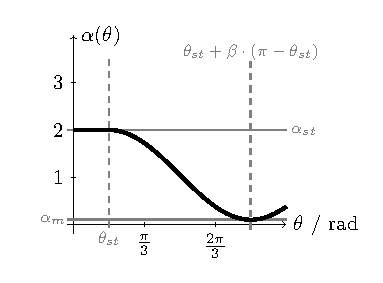
\includegraphics[width=0.5\textwidth]{micarray_alpha.pdf}} & &\\
& 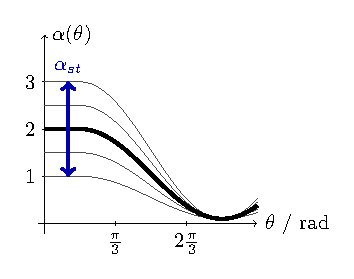
\includegraphics[width=.2\textwidth]{micarray_alpha_st.pdf} & 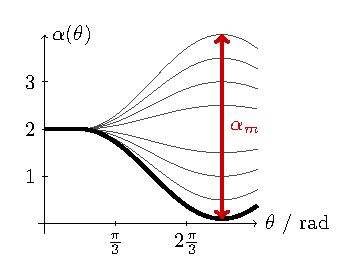
\includegraphics[width=.2\textwidth]{micarray_alpha_m.pdf}\\
& 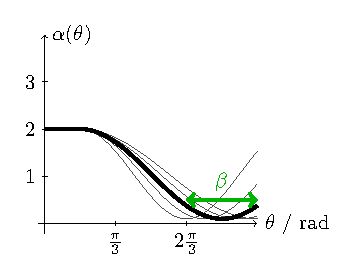
\includegraphics[width=.2\textwidth]{micarray_theta_m.pdf} & 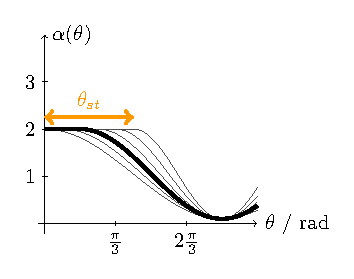
\includegraphics[width=.2\textwidth]{micarray_theta_st.pdf}\\
(a) Exemplary course of $\alpha(\theta)$. & \multicolumn{2}{c}{(b) Influence of each parameter on~$\alpha(\theta)$.}\\
\end{tabular}
 \caption{Relation between design parameters and course of the function $\alpha(\theta)$.}
 \label{Tab_alpha}
\end{center}
\end{table}

Table \ref{Tab_alpha} shows how the four parameters \indattr{alpha\_st}, \indattr{alpha\_m},
\indattr{theta\_st} and \indattr{beta} of this filter type can be used to vary the course of
the design function and thus the spatial design of the filter.
Furthermore, the frequency \indattr{omega} is an additional parameter of this filter
type. By varying the frequency \indattr{omega} the position of the pole and the zero are
varied and the range in which the high-shelf is applied is adjusted.
Moreover, the orientation \indattr{axis} of the filter can be chosen freely. The angle
$\theta$ is then computed with respect to the specified orientation \indattr{axis}.

\definecolor{shadecolor}{RGB}{255,230,204}\begin{snugshade}
{\footnotesize
\label{attrtab:filterhighshelf}
Attributes of filter element {\bf highshelf}\nopagebreak

\begin{tabularx}{\textwidth}{l>{\raggedright}XX}
\hline
name & description (type, unit) & def.\\
\hline
\hline
\indattr{alpha\_m} & alpha at theta = beta*(pi-theta\_st)(double) & nan\\
\hline
\indattr{alpha\_st} & alpha for all theta < theta\_st(double) & nan\\
\hline
\indattr{axis} & orientation axis for filter parameter variation relative to receiver orientation(pos) & 0 0 0\\
\hline
\indattr{beta} & parameter to determine angle at which alpha = alpha\_m(double) & nan\\
\hline
\indattr{omega} & cut-off frequency of high-shelf(double, Hz) & nan\\
\hline
\indattr{theta\_st} & angle at which the zero position starts to vary(double, rad) & nan\\
\hline
\indattr{type} & filter model type(string) & \\
\hline
\end{tabularx}
}
\end{snugshade}



ii) A Parametric Equalizer (\indattr{equalizer})

With the aid of a second-order parametric equalizer a cut or boost can be created around
a certain center frequency. The spatial design of the parametric equalizer is a continuous
variation in center frequency and gain. The design is defined with respect to a freely
selectable orientation \indattr{axis}.
The gain \indattr{gain\_st} is applied in the direction of this orientation \indattr{axis}.
Moreover, the gain of the parametric equalizer is equal to \indattr{gain\_end} at the angle
\indattr{theta\_end}. The gain is continuously varied in between.
The center frequency of the parametric equalizer is continuously varied between the starting
value \indattr{omega\_st} at the orientation \indattr{axis} and the end value
\indattr{omega\_end} at the angle \indattr{theta\_end}.

\definecolor{shadecolor}{RGB}{255,230,204}\begin{snugshade}
{\footnotesize
\label{attrtab:filterequalizer}
Attributes of filter element {\bf equalizer}\nopagebreak

\begin{tabularx}{\textwidth}{l>{\raggedright}XX}
\hline
name & description (type, unit) & def.\\
\hline
\hline
\indattr{Q} & quality factor (double) & nan\\
\hline
\indattr{axis} & orientation axis for filter parameter variation relative to receiver orientation (pos) & 0 0 0\\
\hline
\indattr{gain\_end} & gain applied for all theta >= theta\_end (double, dB) & nan\\
\hline
\indattr{gain\_st} & gain applied at theta = 0 rad (double, dB) & nan\\
\hline
\indattr{omega\_end} & center frequency for theta >= theta\_end (double, Hz) & nan\\
\hline
\indattr{omega\_st} & center frequency at theta = 0 rad (double, Hz) & nan\\
\hline
\indattr{theta\_end} & angle until which the gain is varied (double, rad) & nan\\
\hline
\indattr{type} & filter model type (string) & \\
\hline
\end{tabularx}
}
\end{snugshade}



It can be chosen between two delay models:

i) Free-Field (\indattr{freefield})

This delay model determines the delay between two microphones in the free field.

ii) Sphere (\indattr{sphere})

This delay models the delay of a microphone positioned on a sphere. The used formula is
the model proposed by \citet{BrownDuda} for modeling the interaural time delay for the
Spherical Head Model.

\begin{table} [H]
\begin{center}
\begin{tabular}{c c c}
$\tau = \cfrac{d\cdot \cos\theta}{c}~f_s~\forall~\theta$ &
$\tau_1 = \cfrac{r\cdot \cos\theta}{c}~f_s~\forall~\theta<\cfrac{\pi}{2}$ &
$\tau_2 = \cfrac{r\cdot(\theta-\frac{\pi}{2})}{c}~f_s~\forall~\theta\geq\cfrac{\pi}{2}$\\ 
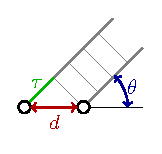
\includegraphics[width=.3\textwidth]{micarray_free_field.pdf} &
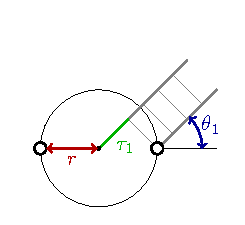
\includegraphics[width=.3\textwidth]{micarray_sphere1.pdf} &
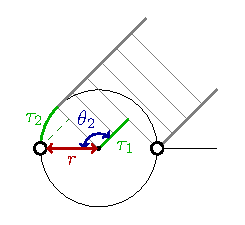
\includegraphics[width=.3\textwidth]{micarray_sphere2.pdf}\\
(a) Free-field & \multicolumn{2}{c}{(b) Sphere}
\end{tabular}
\caption{Used formulas and graphical representation of the delay models.}
\label{Tab_delaymodels}
\end{center}
\end{table}

Table \ref{Tab_delaymodels} shows the graphical representation as well as provides the used
formulas for the computation of the delay models. The delay model is always applied with
respect to the parent microphone.

\definecolor{shadecolor}{RGB}{255,230,204}\begin{snugshade}
{\footnotesize
\label{attrtab:receivermicarray}
Attributes of receiver element {\bf micarray}, inheriting from \hyperref[attrtab:receiver]{{\bf receiver}}\nopagebreak

\begin{tabularx}{\textwidth}{l>{\raggedright}XX}
\hline
name & description (type, unit) & def.\\
\hline
\hline
\indattr{c} & speed of sound(double, m/s) & 340\\
\hline
\end{tabularx}
}
\end{snugshade}


\definecolor{shadecolor}{RGB}{255,230,204}\begin{snugshade}
{\footnotesize
\label{attrtab:mic}
Attributes of element {\bf mic}\nopagebreak

\begin{tabularx}{\textwidth}{l>{\raggedright}XX}
\hline
name & description (type, unit) & def.\\
\hline
\hline
\indattr{delay} & delay line model type, "freefield" or "sphere" (string) & freefield\\
\hline
\indattr{name} & microphone label (string) & \\
\hline
\indattr{position} & microphone position relative to receiver origin (pos, m) & 0 0 0\\
\hline
\indattr{sincorder} & Sinc interpolation order of delay line (double) & 0\\
\hline
\indattr{sincsampling} & Sampling of sinc table, or 0 for direct calculation (uint32) & 64\\
\hline
\end{tabularx}
}
\end{snugshade}


